\documentclass[11pt]{article}
\usepackage[margin=1.6in]{geometry}
\usepackage{amsmath, amssymb}
\usepackage{mathpartir}
\usepackage{listings}
\usepackage{fancyvrb}
\usepackage{color}
\usepackage{bussproofs}
\usepackage{graphicx}
\usepackage{pgf, tikz}
\usetikzlibrary{arrows, automata}

\fvset{%
  fontsize=\small,
  numbers=left
}

\makeatletter
\renewcommand{\Pr}[1]{\text{\textbf{Pr}}\left(#1\right)}
\renewcommand\subsection{\@startsection{subsection}{2}%
  \z@{-.5\linespacing\@plus-.7\linespacing}{.5\linespacing}%
  {\normalfont\scshape}}
\renewcommand\subsubsection{\@startsection{subsubsection}{3}%
  \z@{.5\linespacing\@plus.7\linespacing}{-.5em}%
  {\normalfont\scshape}}
\makeatother

\title{Urbanization in Shanghai}
\author{%
Arissa Li\\
Evan Bergeron\\
Lillian Cho\\
Tiffany Lee
}
\date{\today}

\begin{document}
\maketitle
\section{NYC vs Shanghai: Urban Heat Island}

With global warming forecasts set to continue into the near and
no-so-near future, heat waves will become more and more likely to
occur over time. The Urban Heat Island metric (or UHI for short) is
typically defined as the temperature difference between urban,
suburban, and exurban areas. For instance, \cite{Tan2010} found that
over the last 30 years in Shanghai, the average mid-summer temperature
in urban districts has been increasing at an average rate of 0.073 K
per year, whereas surrounding exurban areas saw no substantial
change. That's a combined increase of urban mid-summer temperature by
more than 2 K.

Comparing results detailed in \cite{Gaffin2008} and \cite{Tan2010}, it
would appear that the UHI effect in NYC is still much more pronounced
than in Shanghai, though Shanghai is quickly catching up. This is a
pattern we see again and again. The majority of years between 1975 and
2010 saw a UHI intensity of roughly 2 to 2.5 K in NYC, with a handful
of years approaching 3 K. In Shanghai, we see an increase from a UHI
of 0.2 K in 1975 to a UHI of 1 K in 2000, with most of the 1990s
having a UHI of roughly 0.8 K.

According to \cite{Xia2014}, we have the following figures. We can see
that air quality and GDP growth are negatively correlated.

\begin{tabular}{cc}
  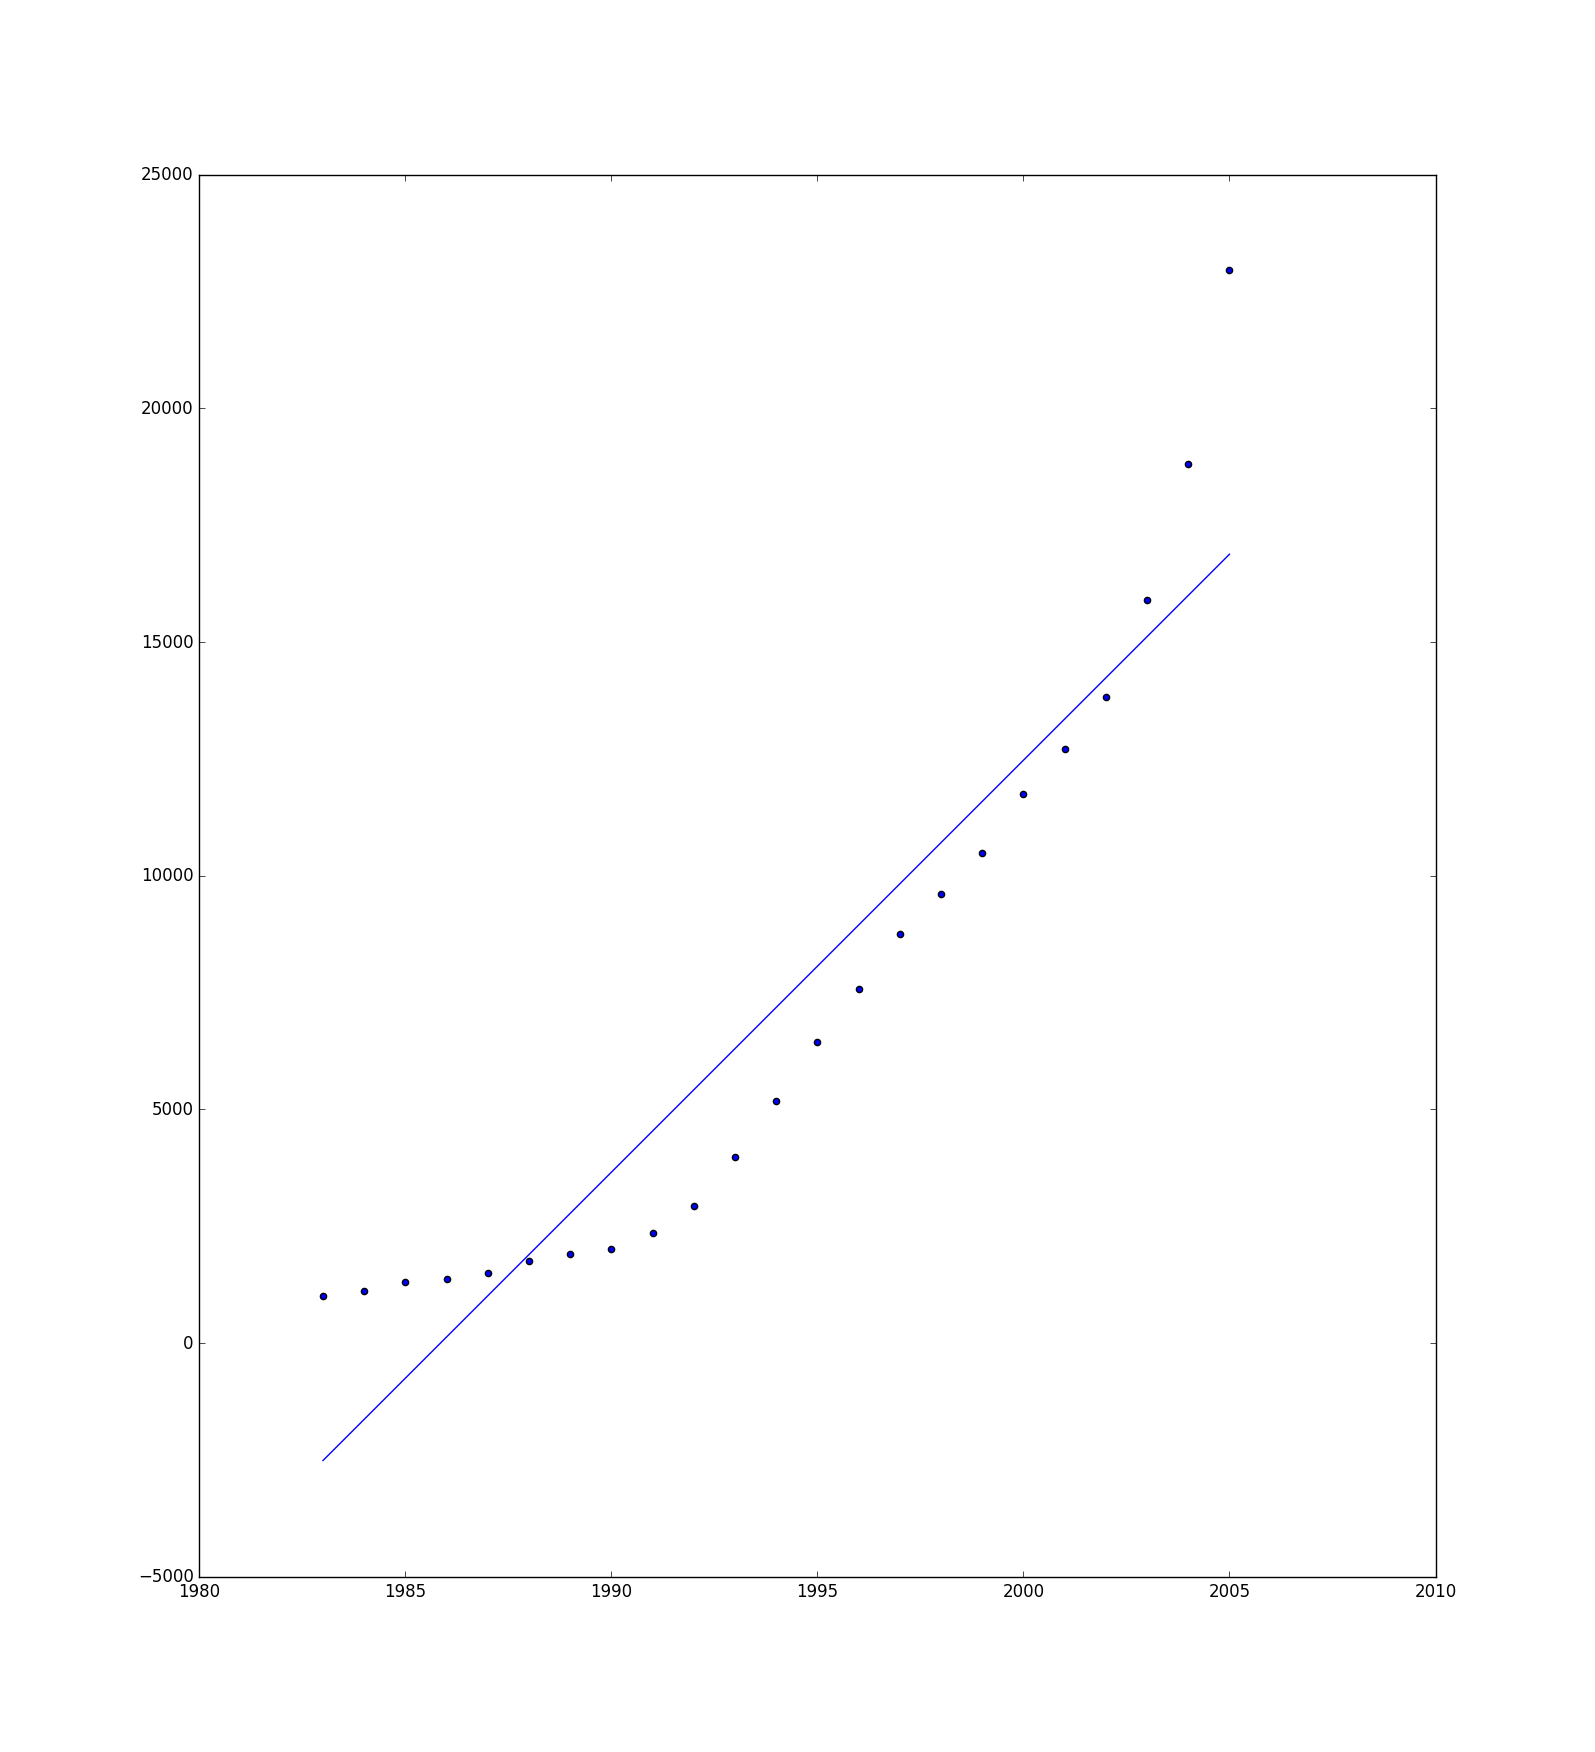
\includegraphics[width=0.5\textwidth]{img/growth_gdp}
& 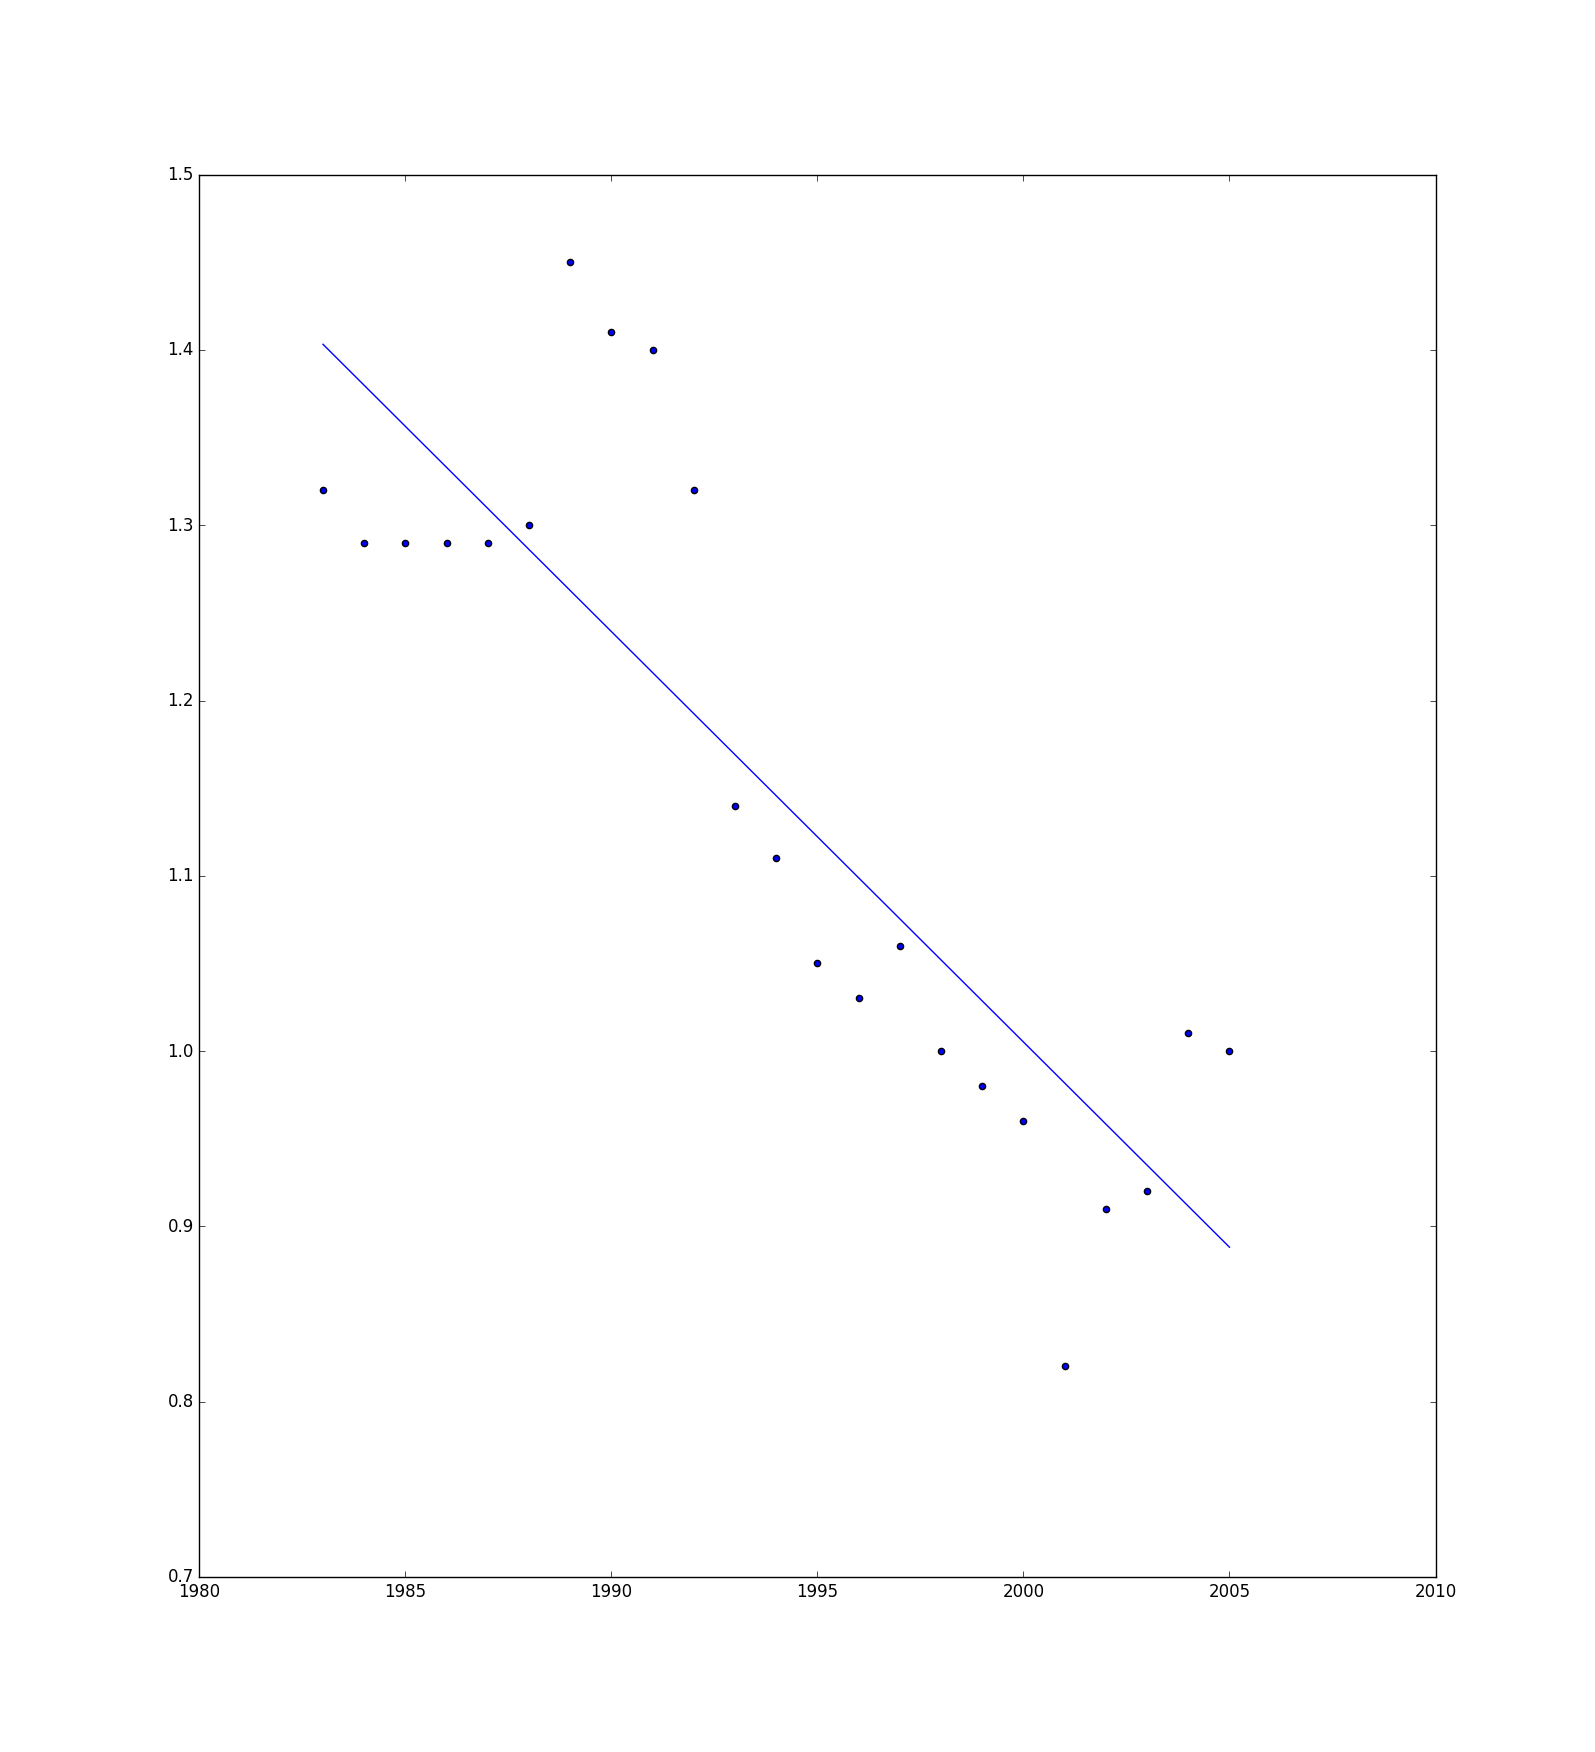
\includegraphics[width=0.5\textwidth]{img/air_quality}\\
   GDP growth over time & Air quality over time 
\end{tabular}

\begin{tabular}{cc}
  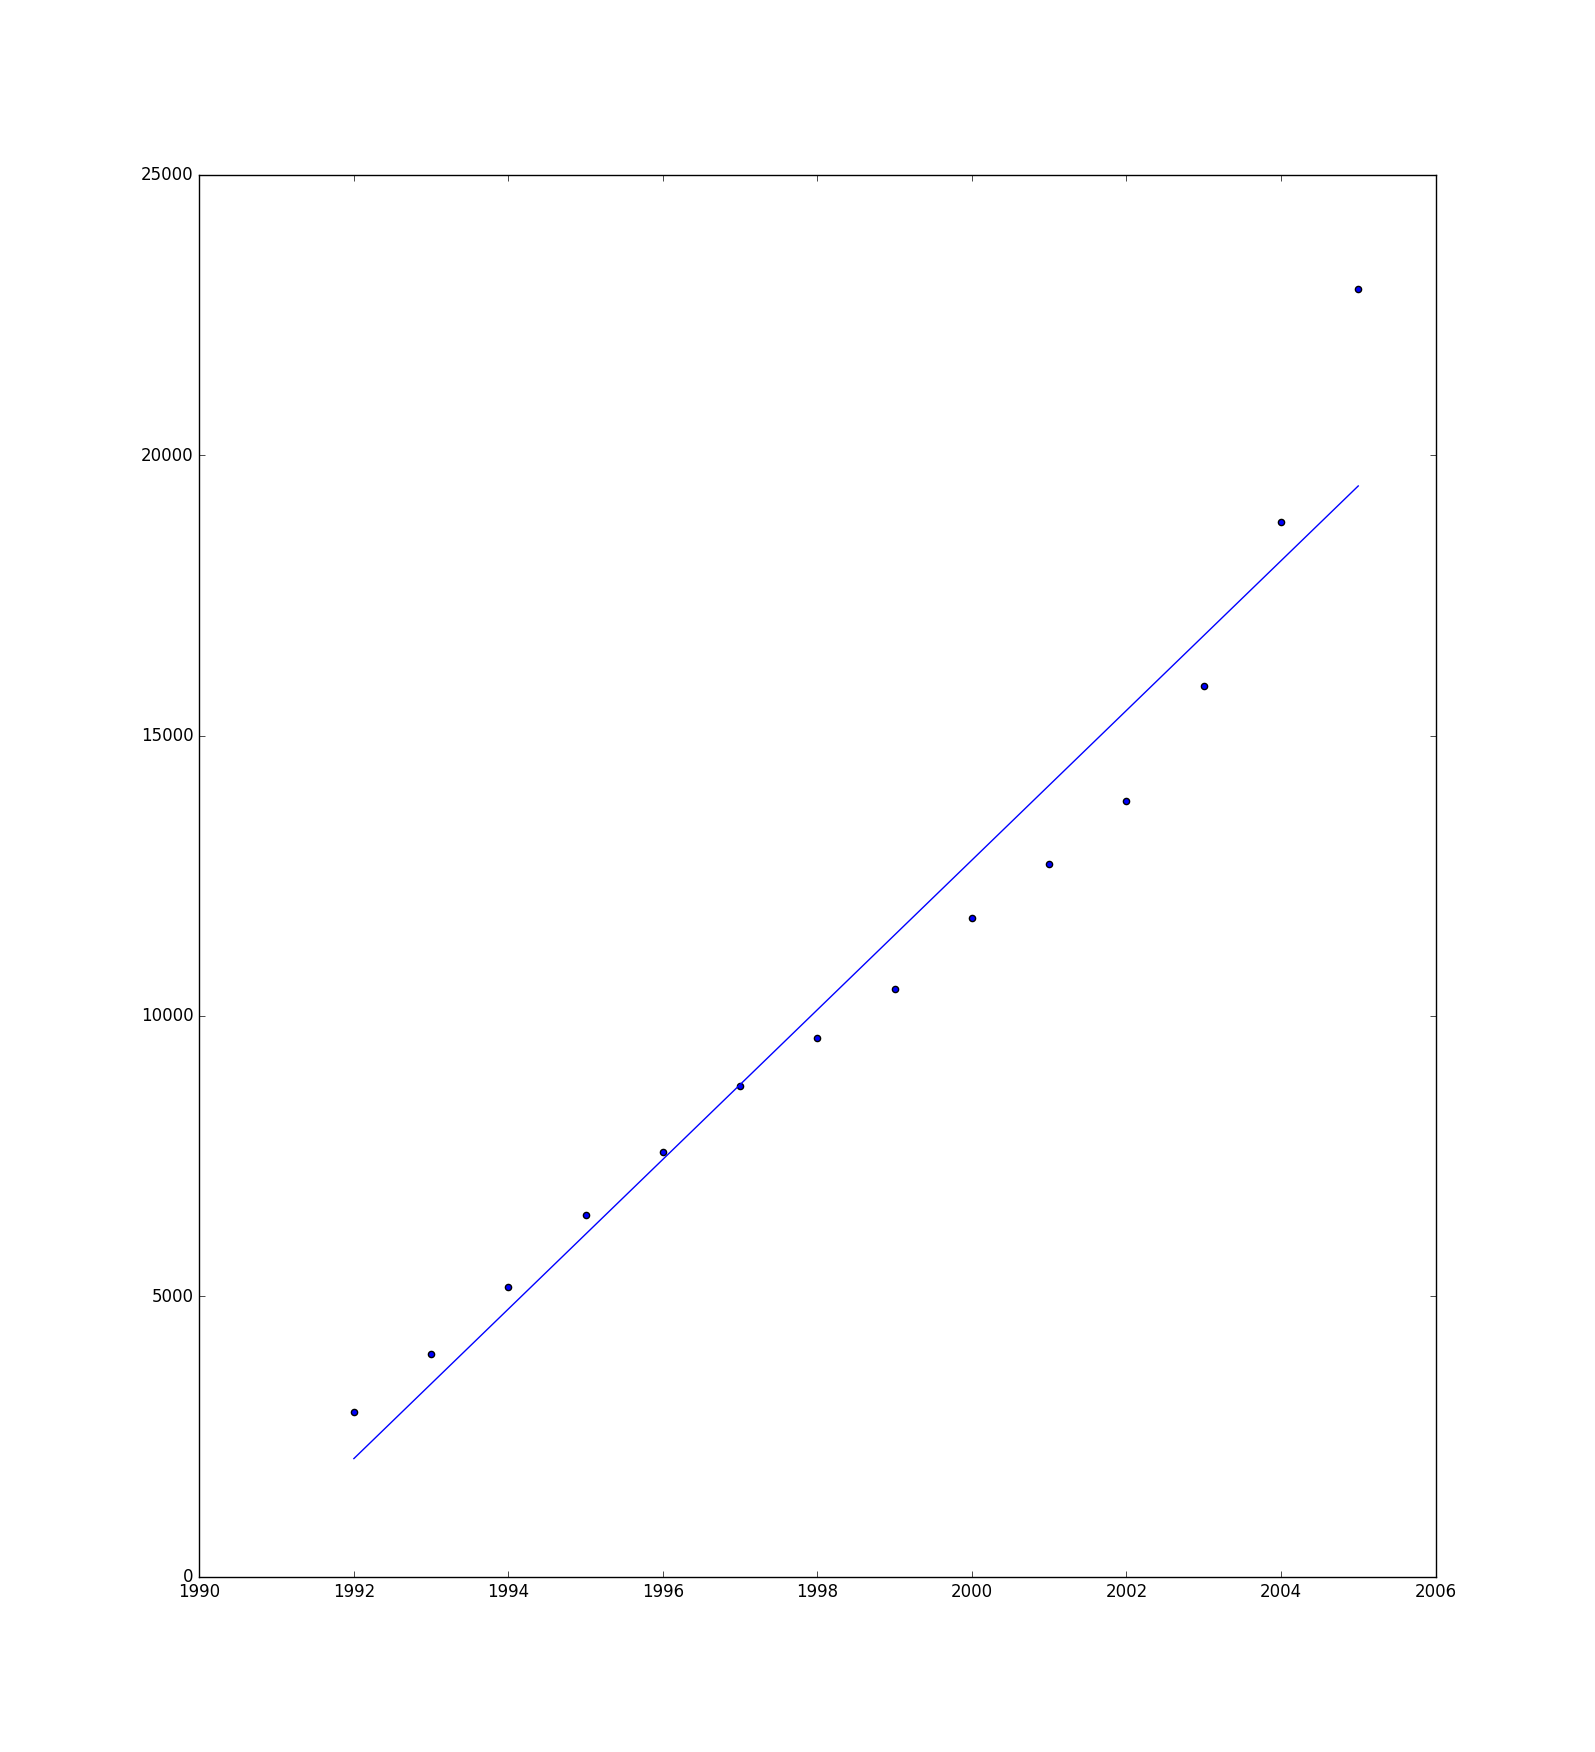
\includegraphics[width=0.5\textwidth]{img/growth_gdp_1991}
& 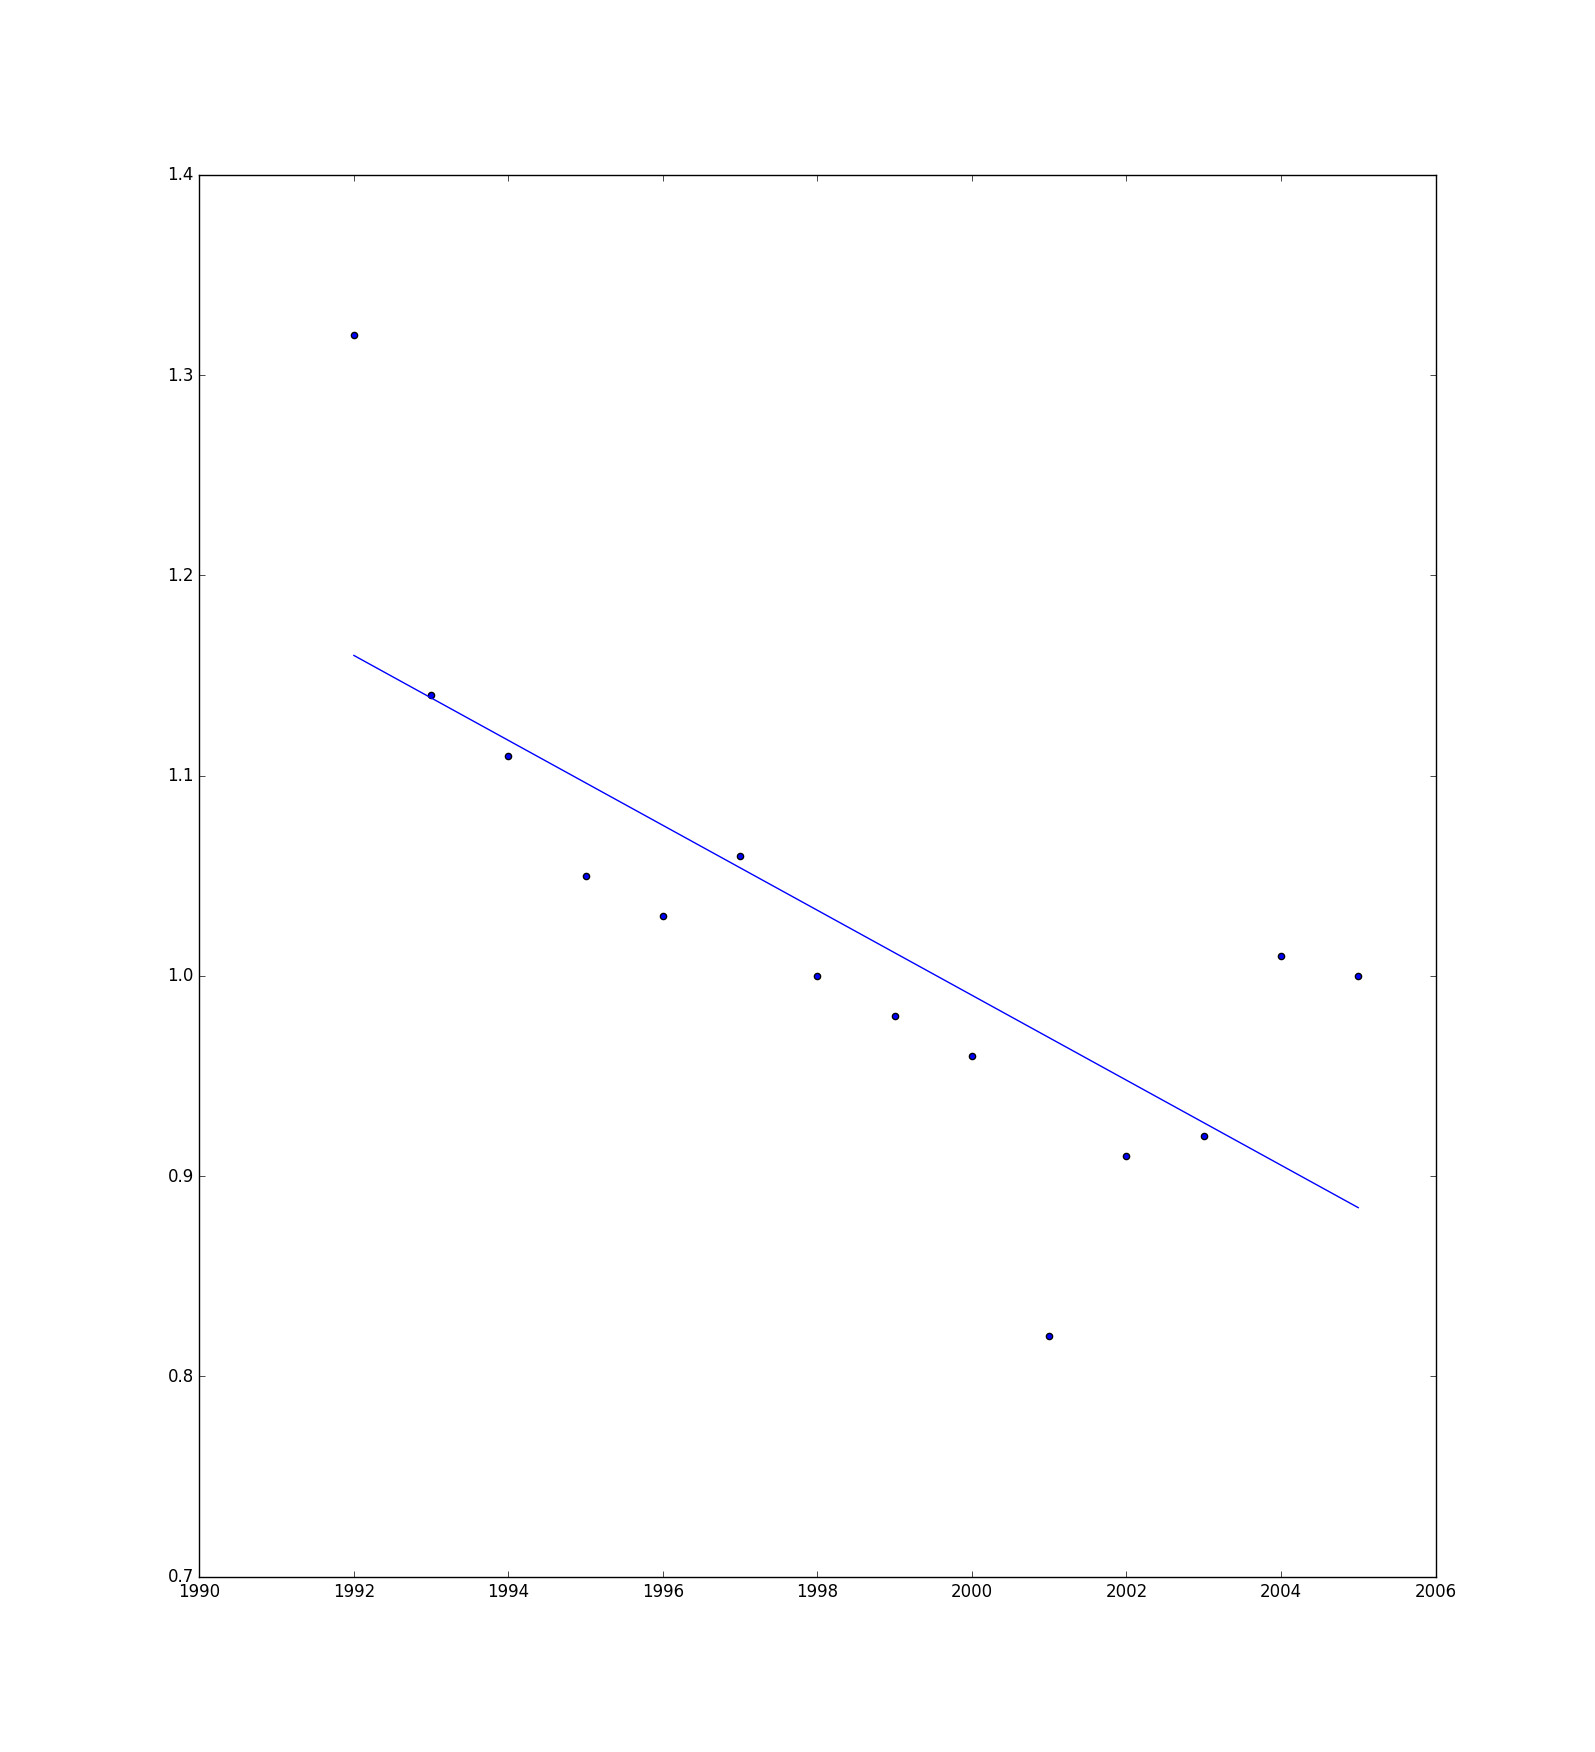
\includegraphics[width=0.5\textwidth]{img/air_quality_1991}\\
   GDP growth since 1991 & Air quality since 1991
\end{tabular}

% bib stuff
\nocite{*}
% \addtocontents{toc}{\protect\vspace{\beforebibskip}}
\addcontentsline{toc}{section}{\refname}
\bibliographystyle{plain}
\bibliography{paper}
\end{document}
